\documentclass[tesis.tex]{subfiles}
\begin{document}
    
\section{Discussion}

Cosas a explicar (discutir que hubiese pasado si esto es diferente).

\textit{Para mí el capitulo fundamental. Los resultados son analizados en detalle, pudiendo incorporar análisis adicionales que no estaban inicialmente en la metodología, como para entender, entre otras cosas, la sensibilidad de los resultados ante parámetros por ejemplo. O la comparación con resultados de otros estudios, o conocimiento existente. En este capítulo se debe entender si lo que se hizo es útil o no.}

\subsection{Estuarine structure and morphology}

During the winter of 2012 Pescadero estuary received less freshwater inflow compared to other months throughout the year, leading the inlet to disconnect from the ocean. Pescadero during its closed state function as a stratified coastal lagoon with river runoff forming a surface layer of fresh water and occasionally having tidal inflows of saline water. The orientation of the bay and the shallowness result in the exposure of all the water column to the wind stress events. In this regard, Pescadero shares many physical traits with other bar-built estuaries where the local wind forcing is the dominant driver.\\

Apart from the stratification, there is an along-estuary density gradient between the outlet of the creek and the mouth, due to the constant discharge of freshwater. Near the mouth the upper layer is thinner than in the creek's outlet, probably because the salinity is higher in the mouth due to the waves that are overtopping the sandbar along with upstream continuous freshwater input.\\

The present study analysis reported that the major driver of mixing is wind stress and the major driver of water level variability is freshwater inflow, even in periods when is very low. In the next sections we are going to discuss the role of other factors that affect Pescadero and its importance in stratification and water level.\\

\subsection{Analysis methods}

Wind and estuarine velocities were axis-rotated in the direction of maximum variance of water currents (See Fig. \ref{fig:rotacion}, Section \ref{Estuary_currents}). This puts the main focus in the estuary currents instead of the wind velocity, but in this particular case, both, wind and water velocities, have a similar principal direction, so it wouldn't be a big difference between each option.\\

We adjusted the first cell of the ADCP data by a visual inspection, using the blank space given by the ADCP, that was 0.71 m, and overlapping it with the CTD data on the same location DC. This comparison gave us the value of 0.91 m for the first cell location, which is a merely estimation, so it could have been a different value, bigger or smaller depending in how we had place the overlapping. This does not affect velocity values, but we have to consider it for the positions of the layers or for the profiles, but it does not make an important change in the analysis.\\

The closed state definition was set in a range of depth's change in time values with a 10 hour frame. The frame was selected by trial and error based on the timescale we were working on and it could change depending on the period in which the data was collected and in the data collection frequency. Also we have to consider that the opening and closures do not happen on an instant, but in a process that could last from minutes to hours, so it could be considered any instant during that process.\\ 

In this study we did not considered temperature and evaporation factors. We considered that the efect of temperature was not important due to the haline stratification that dominated the estuary, but it could be studied in greater depth in future analyzes carried out in Pescadero. Also, we didn't consider evaporation as a factor in depth changes because we are studing an estuary with small area and as it was winter time the air temperature was not too hight to cause mayor impacts.\\

To calculate wind stress we used a drag coefficient defined by \cite{large1981open}, but according to \cite{paugam2021wind} the drag coefficient $C_D$ can be difficult to estimate in shallow water, so we have to consider the obtained $C_D$ as an aproximation in wind stress and everything calculated with that coefficient. In future studies there could be used other drag coefficients to observe if there is a big difference in wind stress and other indices obtained with $C_D$.\\

The Wedderburn number was obtained with the equation for a rectangular basin defined by \cite{Monismith1985}, so it is showing us an approximated value. Despite this, it is still a good indicator to estimate the behavior of the stratification to the wind stress. We could try in future research more adapted Wedderburn numbers to Pescadero basin and compare the results with the obtained in this study.\\

The frequency spectral analysis only show a general view of the most important frequencies in the dataset, but does not show the specific time when this happens. This make it an special tool to detect fequency peaks and contrasts different datasets.\\

\subsection{Changes in Pescadero over time}

\subsection{Wind stress mixing}

Sporadic abrupt changes in density along the water column in different locations were apparent during the periods of closed state. This abrupt changes indicate that they were not caused by gradual processes, but rather resulted from sporadic events that are attributed to the effects of wind stress present at the same time as the density changes. After this events, density did not return to its original values from before the event so mixing was present in the three studied locations.\\

Fig. \ref{fig:perfiles2} is showing density profiles in the studied locations before (in red) and after (in cyan) a big wind event, showing a difference in the density values specially in the bottom where there is a decrease in density. Buoyancy frequency showed a decreased after the wind event meaning a change in stratification same as potential energy anomaly in Fig. \ref{fig:phi}. Also in Fig. \ref{fig:diff} $\Delta \rho/\Delta z$ is showing a decrease in stratification between before and after big wind events, only observing this abrupt change twice, one time during each closed state period.\\

Wedderburn number showed that the lower layer upwelled to the surface during the wind events previously mencioned (Fig. \ref{fig:wedd}). During this mencioned full upwelling event there is the presence of baroclinic presure gradients

On the other hand, 
- And H hat, dH hat/dx and wavelet show when wind is acting in the surface.
 
\subsection{Wind-driven circulation}

- There are water currents provoked by wind stress.

- Wind is the main driver of hydrodynamic changes

- El rango del ADCP no muestra la capa superior

- Cuando sopla el viento la capa superior se desplaza hacia el fondo del estuario y no es detectado por los sensores.

* Imagen de rango ADCP (articulo congreso)
* Velocidad en un wind events
* Dinamica del estuario en el tiempo (Apendice?)

El ADCP no detecta la velocidad de la superficie porque los sensores se encuentran al principio del estuario, lo que genera que la capa superior sea mucho mas delgada que al fondo del estuario.
Esto se puede mostrar con el esquema en katopodes ch11.



% Discutir esta frase de los resultados: Then, when the wind stopped the estuary went stratified with similar values of density to the first profiles, but the velocity had a different behavior, and went negative in the upper layer, probably showing that the water is returning to its original state or that when wind stress is too small the surface water that goes into the same direction of the wind gets thicker and starts to be detected by the ADCP.

\begin{figure}[h!]
    \centering
    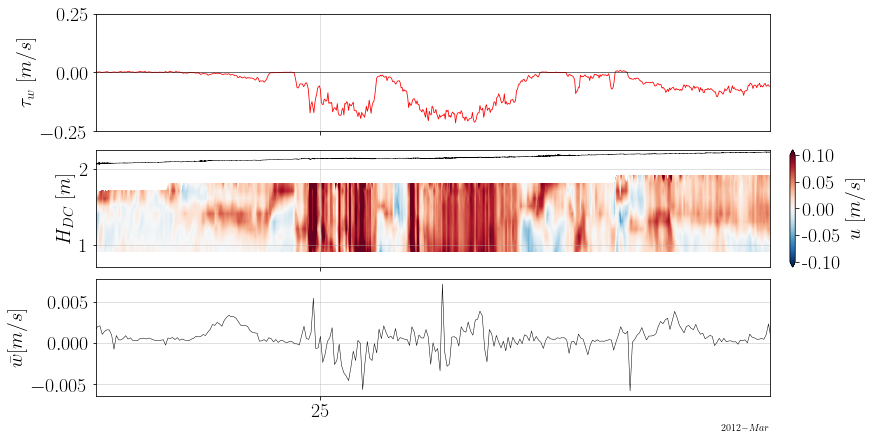
\includegraphics[width=\textwidth]{Imagenes/vel_wind.png}
    \caption{Along-estuary velocity }
    \label{fig:velwind}
\end{figure}

\subsection{Freshwater input}

- Se observa un density decrease en el tiempo

- Se puede ver en rho y en d rho/dz 

- Tal vez se muestra en phi y W por sus cambios en el tiempo (cada vez el viento afecta menos al estuario)

- Su efecto podria estar trabajando en conjunto con el viento para desestratificar el estuario o solo podria estar afectando el viento o solo el caudal

- La teoria que solo el caudal afecta se podria descartar por el primer evento de viento del segundo periodo donde sin aumento de caudal hay un cambio en la estratificacion.

- La teoria que solo el viento afecta se descarta con la disminucion constante de la densidad en el estuario.

- Por otro lado, cuando hay aumento de caudal podria haber mezcla en el estuario debido a que el agua entra con mayor velocidad al estuario.

- Es se observa que provoca cambios solo en la superficie y no tanto en la densidad (H hat, dh/dt, DH hat/Dx, Q)

- Es posible que estos cambios abruptos en la cantidad de caudal entrante generen mezcla, aunque no hay evidencia suficiente para decir que esto esta ocurriendo.

- Al mismo tiempo que hay aumentod de caudal hay Wave overtopping, por lo que no se puede atribuir los cambios en H hat, dh/dt, DH hat/Dx al efecto del aumento del caudal enteramente, pero es probable que si sea porque no se ve algo parecido en los demas eventos de wave overtopping.

* Grafico de tau, H hat, Wavelet, rho, D rho/Dz, Q entre el 13-Feb y 17-Feb

\begin{figure}[h!]
    \centering
    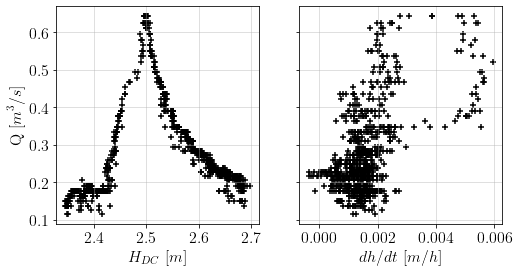
\includegraphics[width=\textwidth]{Imagenes/qh.png}
    \caption{Discharge versus estuary height }
    \label{fig:qh}
\end{figure}


\begin{figure}[h!]
    \centering
    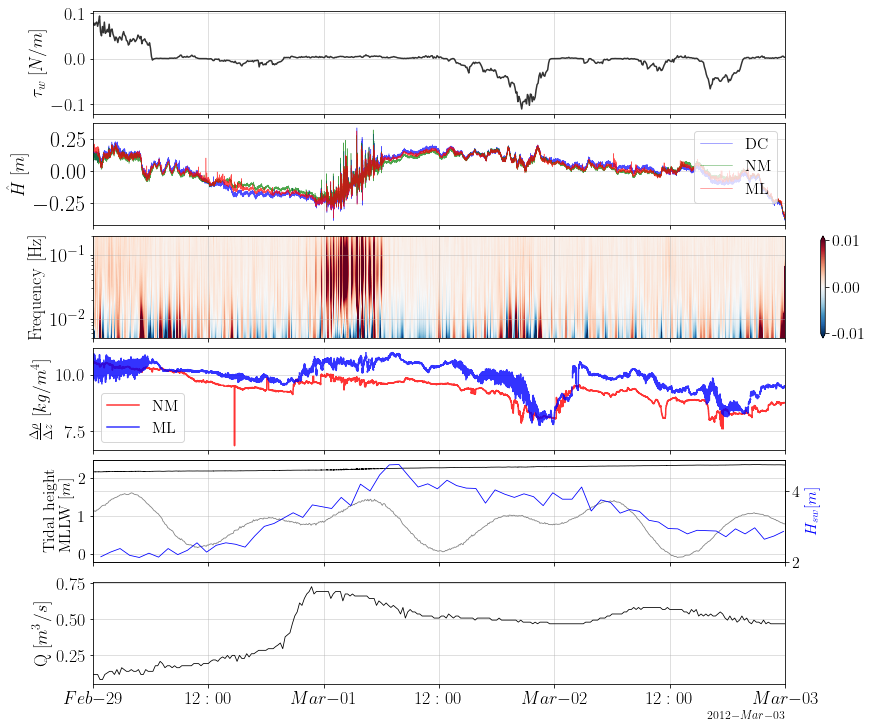
\includegraphics[width=\textwidth]{Imagenes/mix_q.png}
    \caption{ddfsdfsdf }
    \label{fig:mix_q}
\end{figure}

\subsection{Wave overtopping}

- There could be presence of density increase due to wave overtopping 

- In results section we observed some small changes in desnity after wave overtopping 

- Menos en Dc que vimos cambios en el tiempo en el primer periodo.

* Graficos de tau, rho DC fondo, wavelet, d rho/dt 10-hour-frame, Tide/Pdo/Hsw

Why during wave overtopping the bottom of NM increase and then go to normal
explain the  continuous increase in DC at the bottom

The wavelet analysis shows high-frequency waves when that occurs (Figure 3-D and 3-H), but it could be hiding some insignificant wave overtop events.

- Por otro lado, podría haber mezcla en el estuario debido a la entrada turbulenta de las olas sobre la barra de arena.

- Esto se podría atribuir a que cuando hay wave overtopping se observan fluctuaciones en la superficie (H hat, dh/dt, DH hat/Dx, Q), además de los pequeños cambios observados en la densidad

- igual que para el Caso del caudal las surface fluctuations Pueden Ser indicadores de que hay mezcla

- no hay evidencia que lo respalde.

\begin{figure}[h!]
    \centering
    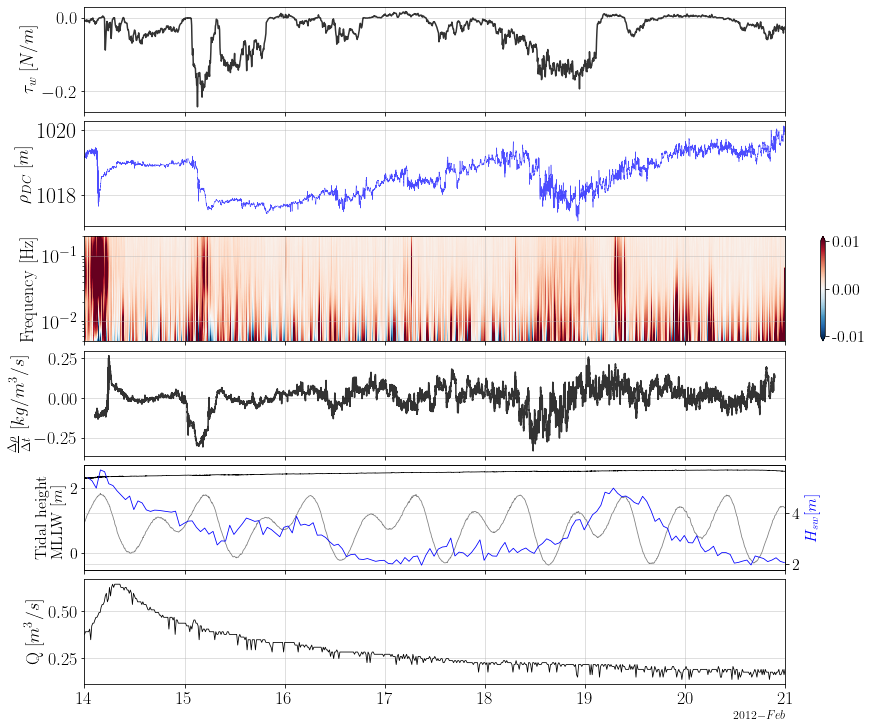
\includegraphics[width=\textwidth]{Imagenes/mix_wo.png}
    \caption{ddfsdfsdf }
    \label{fig:mix_wo}
\end{figure}


\end{document}